%!TEX program = xelatex
\documentclass{book}
\usepackage[a4paper,left=3cm,right=3cm]{geometry}
\usepackage{ctex}
\usepackage{graphics}
\usepackage{graphicx}
\usepackage{multirow}
\usepackage{fancyhdr}
\usepackage{float}  % 避免浮动
\lfoot{} 
	% 这条语句可以让页码出现在下方  
\pagestyle{fancy}
\renewcommand{\headrulewidth}{0pt} 
	% 改为0pt即可去掉页眉下面的横线
\usepackage{verbatim}

\usepackage{listings}	% 代码相关
\usepackage{xcolor}

% \lstdefinestyle{lcustom} {
% 	frame = shadowbox,
% 	numbers = left,
% 	numberstyle = \tiny,
% 	tabsize = 4, 
% 	breaklines = true,
% }

\lstdefinestyle{lfonts}{
	basicstyle   = \scriptsize\ttfamily,
	stringstyle  = \color{purple},
	keywordstyle = \color{blue!60!black}\bfseries,
	commentstyle = \color{olive}\scshape,
}
\lstdefinestyle{lnumbers}{
	numbers     = left,
	numberstyle = \tiny,
	numbersep   = 1em,
	firstnumber = 1,
	stepnumber  = 1,
}
\lstdefinestyle{llayout}{
	breaklines       = true,
	tabsize          = 4,
	columns          = spacefixed,
}
\lstdefinestyle{lgeometry}{
	xleftmargin      = 20pt,
	xrightmargin     = 0pt,
	frame            = tb,
	framesep         = \fboxsep,
	framexleftmargin = 20pt,
}
\lstdefinestyle{lgeneral}{
	style = lfonts,
	style = lnumbers,
	style = llayout,
	style = lgeometry,
}
% \lstset{language = Python, style = lgeneral}
\lstset{style = lgeneral}

\usepackage{tikz}
\usetikzlibrary{mindmap}
\pagestyle{empty}

\usepackage{markdown}
\markdownSetup{smartEllipses = true}
\markdownSetup{hashEnumerators = true}
\markdownSetup{inlineFootnotes = true}
\markdownSetup{fencedCode = true}

\begin{titlepage}
	\title{考研笔记}
	\author{张云涛}
\end{titlepage}

\begin{document}
\maketitle

\tableofcontents

\part{政治}
\chapter*{马克思主义基本原理}


\part{英语}
\chapter*{作文}
九宫格

% Please add the following required packages to your document preamble:
% \usepackage{graphicx}
\begin{table}[]
	\centering
	\resizebox{\textwidth}{!}{%
		\begin{tabular}{|l|l|l|}
			\hline
			话题引起                                                & 图画描述 & 话题概括 \\ \hline
			具体意义                                                & 意义论证 & 意义总结 \\ \hline
			\begin{tabular}[c]{@{}l@{}}归纳总结\\ 预测趋势\end{tabular} & 建议措施 & 憧憬未来 \\ \hline
		\end{tabular}%
	}
\end{table}



\part{数学}
\chapter*{函数极限连续}

\chapter{一元微分}

曲线凹凸性的判断
拐点

驻点

曲率

间断点类型

特殊函数的导数

几何应用
证明应用
物理应用

中值定理

洛尔定理
拉格朗日中值定理
柯西中值定理

关于导数
确定是否为变限积分
比如$sin(x-t)$积分项中含有此式,须设$u=x-t$,或许可化为变限积分,
求导时须注意。

\chapter{一元积分}

\section{概念与性质}

\section{计算}

\section{积分等式与积分不等式}

积分等式
积分不等式


\section{几何应用}

\section{物理应用}

点火公式

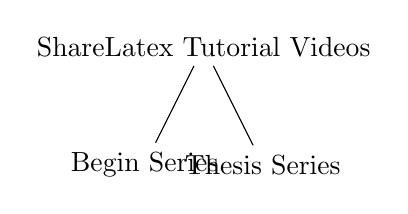
\begin{tikzpicture}
\node{ShareLatex Tutorial Videos}
	child {node {Begin Series}}
	child {node {Thesis Series}}
;
\end{tikzpicture}



% \begin{markdown}
反常积分的判敛,
一次考虑一个奇点,
所以可能会有多个限制范围

\end{markdown}
\chapter{多元微分}


多元微分的题型

\section{概念}
各种术语的概念,及公式。

\noindent
偏导数连续 $\Longrightarrow$ 可微 $\Longrightarrow$ 偏导数存在(某方向双侧) \\
偏导数连续 $\Longrightarrow$ 可微 $\Longrightarrow$ 连续 $\Longrightarrow$ 极限存在(全方向) \\
偏导数存在 $\Longrightarrow$ 可微 $\Longrightarrow$ 方向导数存在(某方向单侧) \\

注
不能用洛必达法则、单调有界准则 \\
$dz = A\Delta x + B\Delta y + o(\rho)$ \\
$dz = A\Delta x + B\Delta y + o(\sqrt{x^2+y^2})$ \\


驻点

\section{复合函数求导}
求导方法
1. 链式求导法则 \\ 
2. 全导数 \\
3. 全微分形式不变性 \\



\section{隐函数求导}
一个方程的情形

方程组的情形
雅克比矩阵,公式法 

方程组简单情形



\section{多元函数的极值、最值}
题型包括条件极值和无条件极值

\subsection{无条件极值}
求解步骤
1. 令偏导数=0, 求得(x,y)
2. 求二阶偏导数
$$
A = f_{11}^{''} \quad{}  B = f_{12}^{''} \quad{} C = f_{22}^{''}
$$
其中若$B^2 - AC < 0$,极值存在,
若$A > 0$,则为极小值,若$A < 0$,则为极大值,
若$A = 0$,则失效,另外计算。


\subsection{条件极值}
运用拉格朗日乘数法,构造
$F(x, y, z, \lambda, \mu) = 0$ \\
分别求偏导数,令其=0, 求得$(x, y, z)$。
优先求$(x, y, z)$。 

\section{偏微分方程}

$z(x,y) = \int f_x^{'}(x,y) dx + \varphi(y)$ \\
代入已知条件求得$\varphi(y)$ \\
求得$z(x,y)$ \\

\chapter{二重积分}

二重积分

求和化为积分

特殊的曲线
及其形状

质心坐标

$$x =\frac{\int\int x d\sigma}{\int \int d\sigma} $$

转动惯量
$$ I_x = \int\int y^2 d\sigma $$


\chapter*{多元积分}

\chapter*{微分方程}

\chapter*{空间几何}

\chapter*{无穷级数}

常数项级数
幂级数
福利叶级数

收敛区间 开区间
收敛半径 R
收敛域   考虑端点



\begin{markdown}

## 级数展开

## 级数求和
先积后导    \\
先导后积

## 傅里叶级数

\end{markdown}


\chapter*{矩阵}

\chapter*{线性方程组}

\chapter*{特征值与特征向量}

\chapter*{二次型}

\chapter{概率统计}
<<<<<<< HEAD
概率统计计34分
=======

概率统计总计34分,重要性较低。
4月24日夜学习方浩教学视频。

\begin{itemize}
	\item 随机事件与概率
	\item 随机变量与分布函数
	\item 多维随机变量
	\item 数字特征
	\item 大数定律与中心极限定理
	\item 数理统计基本概念
	\item 参数估计与假设检验
\end{itemize}


第一章 随机事件与概率
重点内容

事件的关系与运算
几何概型
条件概率、乘法公式、独立性

独立性
仅针对概率而言,与事件无关。

独立性的经验
一般不独立
互斥的一般不独立
包含的一般不独立

两两独立  
相互独立
相互独立要求高 $P(ABC) = P(A)P(B)P(C)$

线代概率 重在理解,不应重心放于计算。


概率的计算主要靠事件的计算
事件的计算主要靠事件的关系

>>>>>>> 6ffde2a84f2eeee4b356b0bc0e57b83e01d37a7b

\chapter{随机变量及其分布}
本章主要两部分内容
分布函数和正态分布

\begin{itemize}
	\item 分布函数
	\item 正态分布
\end{itemize}



\begin{table}
	\centering
	\caption{变量分布}
	\begin{tabular}{|l|l|l|l|}
		\hline
		分布函数 &  &  &  \\ \hline
		0-1分布 &  &  &  \\ \hline
		二项分布 &  &  &  \\ \hline
		泊松分布 &  &  &  \\ \hline
		几何分布 &  &  &  \\ \hline
		超几何分布 &  &  &  \\ \hline
	\end{tabular}
\end{table}

重点考虑泊松分布和几何分布

\chapter*{多维随机变量及其分布}

事件的关系与运算

几何概型

条件概率、乘法公式、独立性

\chapter*{随机变量的数字特征}
  
\chapter{大数定律与中心极限定理}

\chapter*{数理统计基本概念}

\chapter*{参数估计与假设检验}



\part{计算机}
\include{cs/线性表}
\chapter*{栈和队列}

\chapter*{树、二叉树}

\include{cs/图}
\chapter*{查找}

最短路径

关键路径

\chapter*{排序}

十大排序算法

插入排序
交换排序
归并排序
等等

此知识点尚未完全掌握
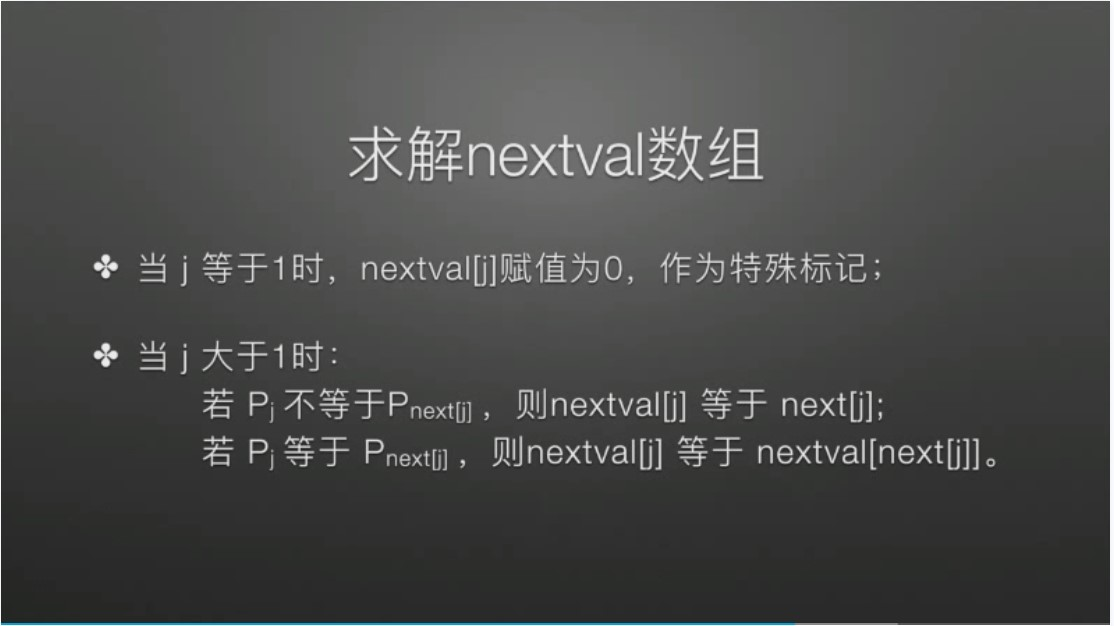
\includegraphics{images/cs/KMPnextval.jpg}

\chapter{进程管理}

操作系统的特征
并发、共享、虚拟、异步
并发是最基本的特征。

处理机管理的主要功能
进程管理、进程同步、进程通信、处理机调度

内存管理的主要功能
内存分配、内存保护、地址映射、内存扩充

设备管理的主要功能
缓冲管理、设备分配、设备处理、虚拟设备

文件管理的主要功能
文件存储空间的管理、目录管理、文件的读写管理和保护

微内核OS
足够小的内核、基于C/S模式、应用机制与策略分离原理、采用面向对象技术

前趋图
有向无循环图,记为DAG,描述进程之间执行的前后关系。

并发是OS的基本特征,进程的重要特征
动态性是进程的基本特征

PCB 进程控制块

进程状态及之间切换
以及各种事件对应的切换
就绪--> 执行 进程分配到CPU资源
执行--> 就绪 时间片用完
执行--> 阻塞 IO请求
阻塞--> 就绪 IO完成

挂起状态
处于挂起状态的进程不能接受处理机调度

引起进程创建的主要事件
用户登录、作业调度、提供服务、应用请求

引起进程撤销的主要事件
正常结束、异常结束(越界错误、保护错、非法指令、
特权指令错、运行超时、等待超时、算术运算错、IO故障)、
外界干预(操作系统敢于、父进程请求、父进程终止)

临界区

同步机制

同步准则
空闲让进、忙则等待、让权等待、有限等待

信号量 wait signal

整型信号量未完全遵守准则,不满足“让权等待”准则

互斥信号量 mutex,初值为1 
 

生产者消费者问题

锁 lock

管程
组成 名称、共享数据结构说明、过程、设置初始值
条件变量 condition 

AND信号量
信号量集

进程通信
低级工具 
高级工具 共享存储、消息传递、管道通信


引入线程
在操作系统中引入线程,是为了减少程序在并发执行时锁付出的时空开销,使OS具有更好的并发性,提高CPU的利用率。
进程是分配资源的基本单位,线程是系统调度的基本单位。

线程属性
轻型实体、独立调度和分派的基本单位、可并发执行、共享进程资源
一个进程的多个线程也可以并发执行



多线程OS中实现进程之间的同步与通信,提供的同步机制
互斥锁、读写锁、条件变量、信号

用户级线程
内核支持线程

高级调度、低级调度、中级调度
作业
作业 作业步 作业流

调度算法

作业调度与进程调度

死锁
产生原因与必要条件
原因 竞争资源和进程间推进顺序非法
必要条件 互斥条件、请求和保持、不可剥夺、循环等待

解决死锁方法
预防、避免、检测和解除
预防最容易实现
避免使资源利用率最高

银行家算法


提问方式
设计避免死锁的方法
解释说明产生死锁的原因和必要条件
NEEP矩阵

管程 是什么、组成、引入原因





\chapter{内存管理}
buddy

对换

分页存储管理
分段存储管理

快表
地址转换

虚拟存储器的特征
多次性、对换性、虚拟性,
虚拟性最本质

页表
页号、物理块号、状态位P、访问字段A、修改位M、外存地址

缺页中断
缺页次数

CLOCK
改进型CLOCK

中断处理过程

共享

\chapter{文件管理}

文件系统的结构及其实现,磁盘相关

文件系统
文件控制块、物理分配方法、索引结构、
磁盘
磁盘特性和结构、磁盘调度算法、磁盘相关性能

文件的逻辑结构
目录结构的实现
系统调用
文件的物理结构
存储空间的管理
文件共享保护

\section{文件系统}

\subsection{文件的逻辑结构}
文件的逻辑结构
	无结构文件(流式文件) 
	有结构文件(记录式文件) 
		顺序文件
			顺序存储或者链式存储
			串结构 顺序结构 
		索引文件
		索引顺序文件

\subsection{目录结构}
FCB的有序集合称为文件目录
一个FCB就是一个文件目录项

索引结点
磁盘索引结点、内存索引结点

引入无环图目录的目的是实现文件共享
无环图 共享计数器 计数器为0时才真正删除该结点


索引结点(FCB的改进)
FCB中暂时不用的信息放入索引结点中

索引结点机制,提升了文件检索速度


% 重点内容 
\subsection{文件物理结构}
即文件分配方式

文件的物理结构/文件分配方式
文件存储空间管理

索引分配
m级访问,m+1次读磁盘(顶级索引表未调入内存的情况下)

链接分配
索引分配

混合索引分配
Unix采用13个地址,0-9 直接地址,10-一级索引,11-二级索引,12-三级索引 

文件目录与目录文件

计算逻辑地址到物理地址的转换,以及查找次数。

文件共享
基于符号链的文件共享
软链接、硬链接


\subsection{文件存储空间管理}

空闲表法
空闲链表法
位示图法 字号,位号  常考 
成组链接法 UNIX超级块 








2020年4月14日凌晨观看王道2020视频教程

\chapter{设备管理}

设备控制器

CPU与设备控制器之间的通信

IO控制

IO控制方式
程序IO方式
中断驱动IO控制方式
直接存储器访问(DMA)IO控制方式
IO通道控制方式

缓冲
引入缓冲的原因

单缓冲 $max(C,T)+M$
双缓冲 $max(C+M,T)$,M短暂可以忽略不计
% 示意图 待插入图示

设备独立性

设备虚拟

SPOOLing技术
输入井、输出井、输入缓冲区、输出缓冲区、输入进程SPi、输出进程SPo

磁盘访问 
磁盘访问时间 寻道时间、旋转延迟事件、传输时间
磁道
磁盘调度算法

磁盘高速缓冲


 

\chapter*{IO管理}



奈氏准则 理想低通 
极限码元传输率 2W Baud
极限数据传输率 2W log2V b/s



\include{cs/数据链路层}
\include{cs/网络层}
\chapter*{传输层}

\chapter*{应用层}

\begin{markdown}
你好亚

### 你好 


\end{markdown}



\end{document}
